\documentclass[border=20pt]{standalone}
% \documentclass[parskip]{scrartcl}
% \usepackage[margin=15mm]{geometry}
\usepackage{tikz}
\usetikzlibrary{calc,shapes,shadows}

\global\edef\lastangle{0}
\newcounter{sectornumber}

\newcommand{\ring}[4]{% angles&colors, inner, outer radius, height
\begin{scope}[x={(0.866cm,0.5cm)},y={(-0.866cm,0.5cm)},z={(0cm,1cm)}]
\global\edef\lastangle{0}
\setcounter{sectornumber}{1}
\foreach \x/\ringcolor in {#1}
{   \pgfmathsetmacro{\na}{\lastangle+\x*3.6}
    \colorlet{darkercolor}{\ringcolor!60!black}
    \colorlet{darkestcolor}{\ringcolor!20!black}
    \shadedraw[top color=darkercolor,bottom color=darkestcolor,draw=darkercolor] (\lastangle:#2) arc (\lastangle:\na:#2) -- ++(0,0,#4) arc (\na:\lastangle:#2) -- cycle;
    \shadedraw[top color=darkercolor,bottom color=darkestcolor,draw=darkercolor] (\lastangle:#3) arc (\lastangle:\na:#3) -- ++(0,0,#4) arc (\na:\lastangle:#3) -- cycle;
    \global\edef\lastangle{\na}
}
\global\edef\lastangle{0}
\foreach \x/\ringcolor in {#1}
{   \pgfmathsetmacro{\na}{\lastangle+\x*3.6}
    \colorlet{darkercolor}{\ringcolor!60!black}
    \colorlet{darkestcolor}{\ringcolor!20!black}
    \fill[\ringcolor,draw=darkercolor] (0,0,#4) ++(\lastangle:#2) arc (\lastangle:\na:#2) -- ++(\na:#3-#2) arc (\na:\lastangle:#3) -- cycle;
    \pgfmathsetmacro{\nodepos}{(#3+#2)*0.5}
    \node (n\thesectornumber) at ($(0,0,#4)+(\lastangle+\x*1.8:\nodepos)$) {};
    \stepcounter{sectornumber}
    \global\edef\lastangle{\na}
}
\end{scope}
}

\begin{document}

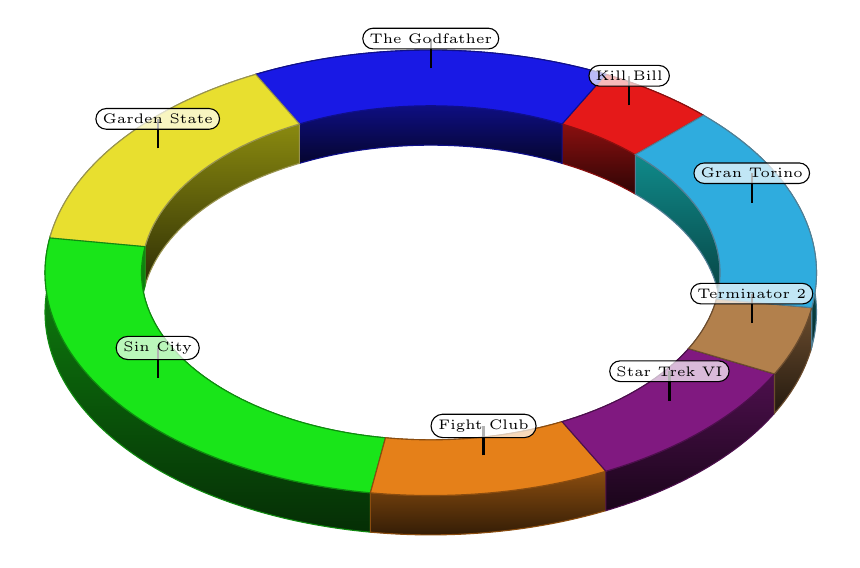
\begin{tikzpicture}
\ring{5/red!80!gray,15/blue!80!gray,15/yellow!80!gray,25/green!80!gray,10/orange!80!gray,10/violet!80!gray,5/brown!80!gray,15/cyan!80!gray}{3}{4}{0.5}
\foreach \x/\label in {1/Kill Bill,2/The Godfather,3/Garden State,4/Sin City,5/Fight Club,6/Star Trek VI,7/Terminator 2,8/Gran Torino}
{   \draw[thick] (n\x) -- ++(0,0.5) node[fill=white,draw,rounded rectangle,inner sep=2pt,thin,fill opacity=0.7,text opacity=1] {\tiny\label};
}
\end{tikzpicture}


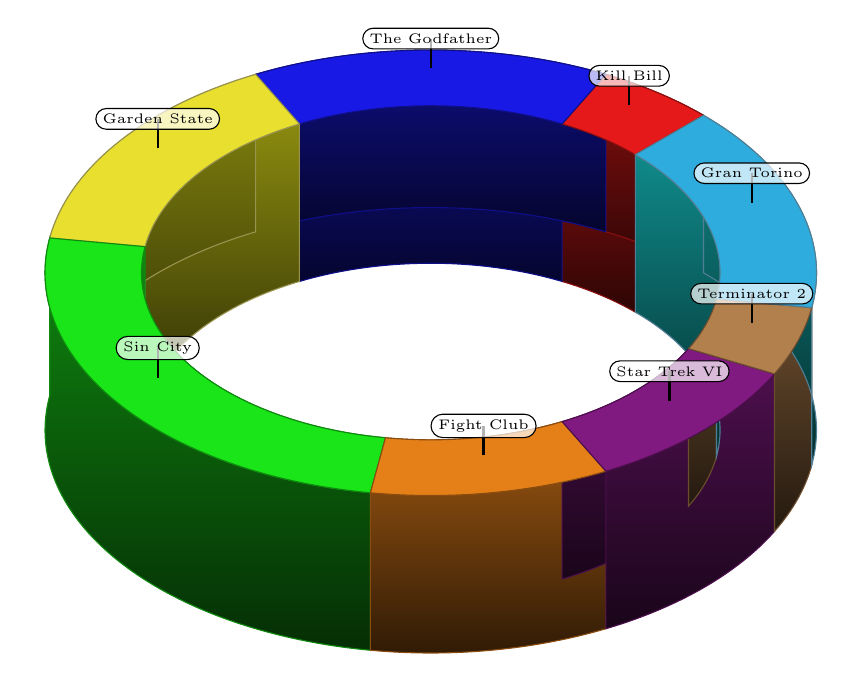
\begin{tikzpicture}[x={(0.866cm,0.5cm)},y={(-0.866cm,0.5cm)},z={(0cm,1cm)}]
\ring{5/red!80!gray,15/blue!80!gray,15/yellow!80!gray,25/green!80!gray,10/orange!80!gray,10/violet!80!gray,5/brown!80!gray,15/cyan!80!gray}{3}{4}{2}
\foreach \x/\label in {1/Kill Bill,2/The Godfather,3/Garden State,4/Sin City,5/Fight Club,6/Star Trek VI,7/Terminator 2,8/Gran Torino}
{   \draw[thick] (n\x) -- ++(0.5,0.5) node[fill=white,draw,rounded rectangle,inner sep=2pt,thin,fill opacity=0.7,text opacity=1] {\tiny\label};
}
\end{tikzpicture}


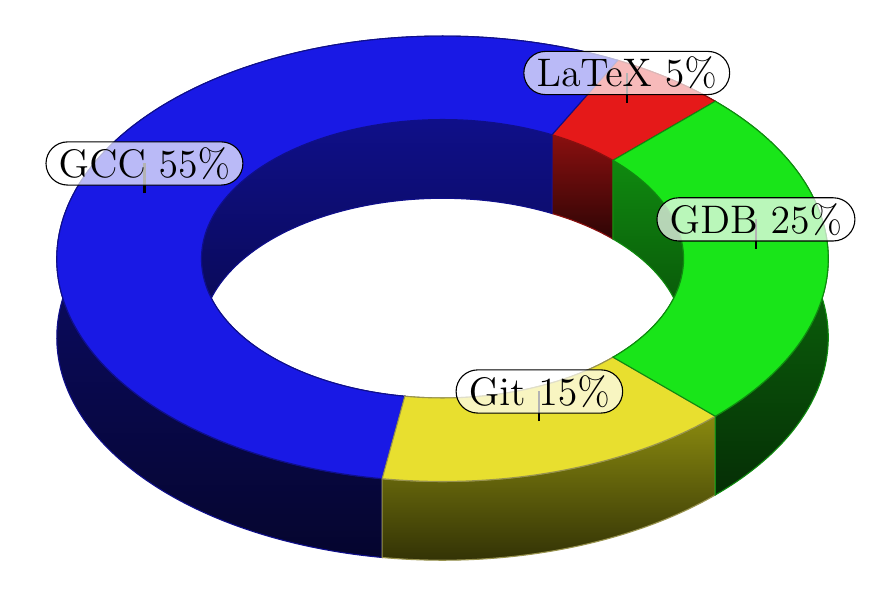
\begin{tikzpicture}
\ring{5/red!80!gray,55/blue!80!gray,15/yellow!80!gray,25/green!80!gray}{2.5}{4}{1.0}
\foreach \x/\label in {1/LaTeX 5\%,2/GCC 55\%,3/Git 15\%,4/GDB 25\%}
{   \draw[thick] (n\x) -- ++(0,0.5) node[fill=white,draw,rounded rectangle,inner sep=2pt,thin,fill opacity=0.7,text opacity=1] {\Large\label};
}
\end{tikzpicture}

\end{document}
